\chapter{Experimental setup}

The exerimental setup was largely adopted from \cite{Hertlein2017}. Amendments
made include the \gls{rf} signal source of the \gls{aod} and an additional
photodiode to measure the deflected beam intensity.

\section{Optics}

The optical setup can be disected into a closed first section that reduces
the power of the $\SI{532}{\nano\meter}$ laser source from $\SI{10}{\watt}$
to below $\SI{2}{\milli\watt}$ and includes an \gls{aom} for intensity
regulation, and an open second section for beam deflection.
Both sections are connected through a \gls{smf}.

\subsection{Power reduction}

Because of safety concerns the power reduction section is confined into a
visually sealed box housing. \Cref{fig:setup_power_reduction} reveals the
inside of the power reduction box.
\begin{figure}[ht]
  \centering
  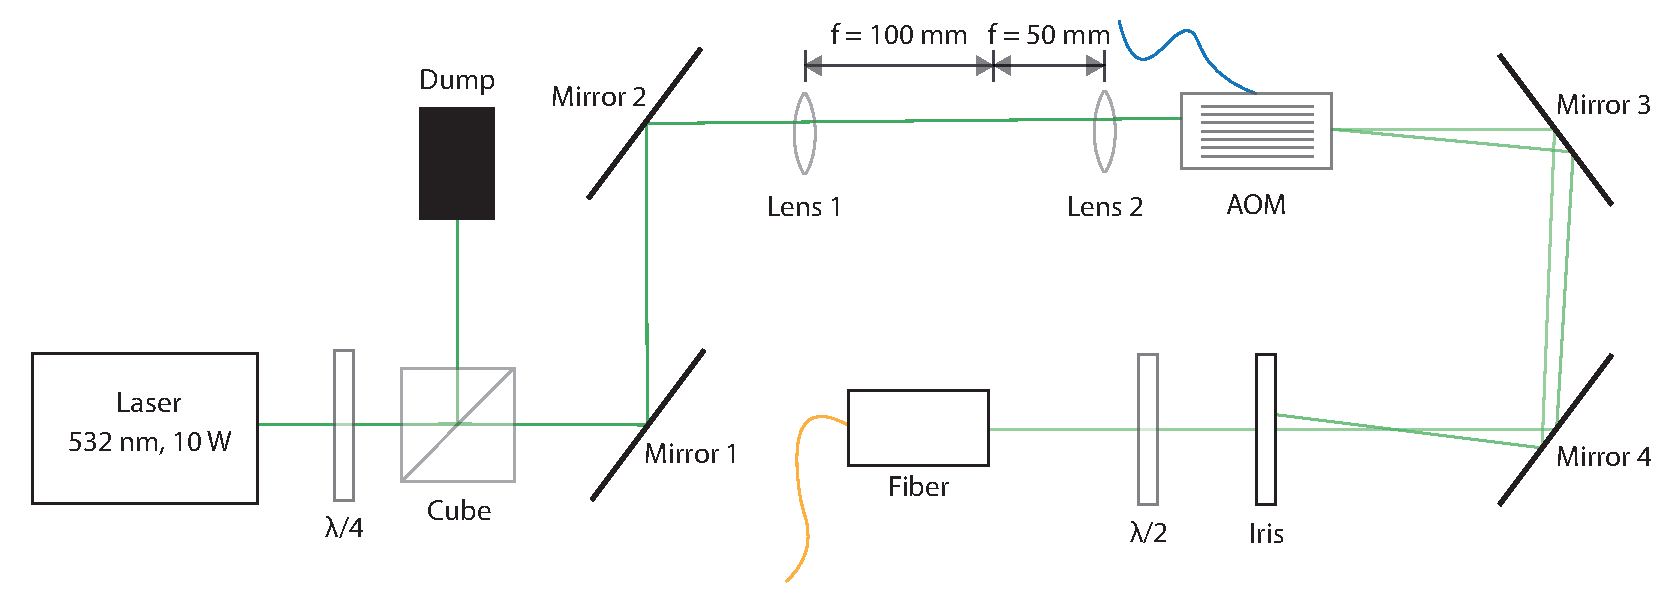
\includegraphics[width=\textwidth]{\figuredir{setup/power-reduction.pdf}}
  \caption{Optical configuration of the power reduction section.
  }\label{fig:setup_power_reduction}
\end{figure}
The laser beam leaving the laser source is polarized by a $\lambda/2$ retarder
plate such that the succeeding high power beamsplitter diverts the majority
of the beam power into a beam dump. Afterwards Mirror 1 and Mirror 2 direct
the beam towards the center of a $2:1$ telescope composed of Lens 1 and
Lens 2. An \gls{aom} diffracts the laser beam into multiple orders. Mirror 3
and Mirror 4 project theses orders onto a pinhole which is configured to
intromit only the first order deflection. The intensity of the first order is
subject to amplitude modulation to the \gls{aom}. Finally a tunable
$\lambda/2$ retarder plate can be used to couple the beam polarization with
the \gls{smf}.

\subsection{Beam deflection and detection}

The section for beam deflection and detection as disclosed in
\Cref{fig:setup_beam_deflection} receives the down-powered laser beam from
previously described section by a \gls{smf}. Hereinafter the beam passes a
tunable retarder plate and beam splitter Cube 1. A second polarizer with
Cube 2 is used to branch off a part of the beam to Photodiode 1 that is
positioned to be at the focal point of lens Lens 1. Photodiode 1 is connected
via a control system with the amplitude modulation of the \gls{aom} depicted
in \Cref{fig:setup_power_reduction} to stabilize the laser intensity against
i.e.\ thermal drifts.
\begin{figure}[ht]
  \centering
  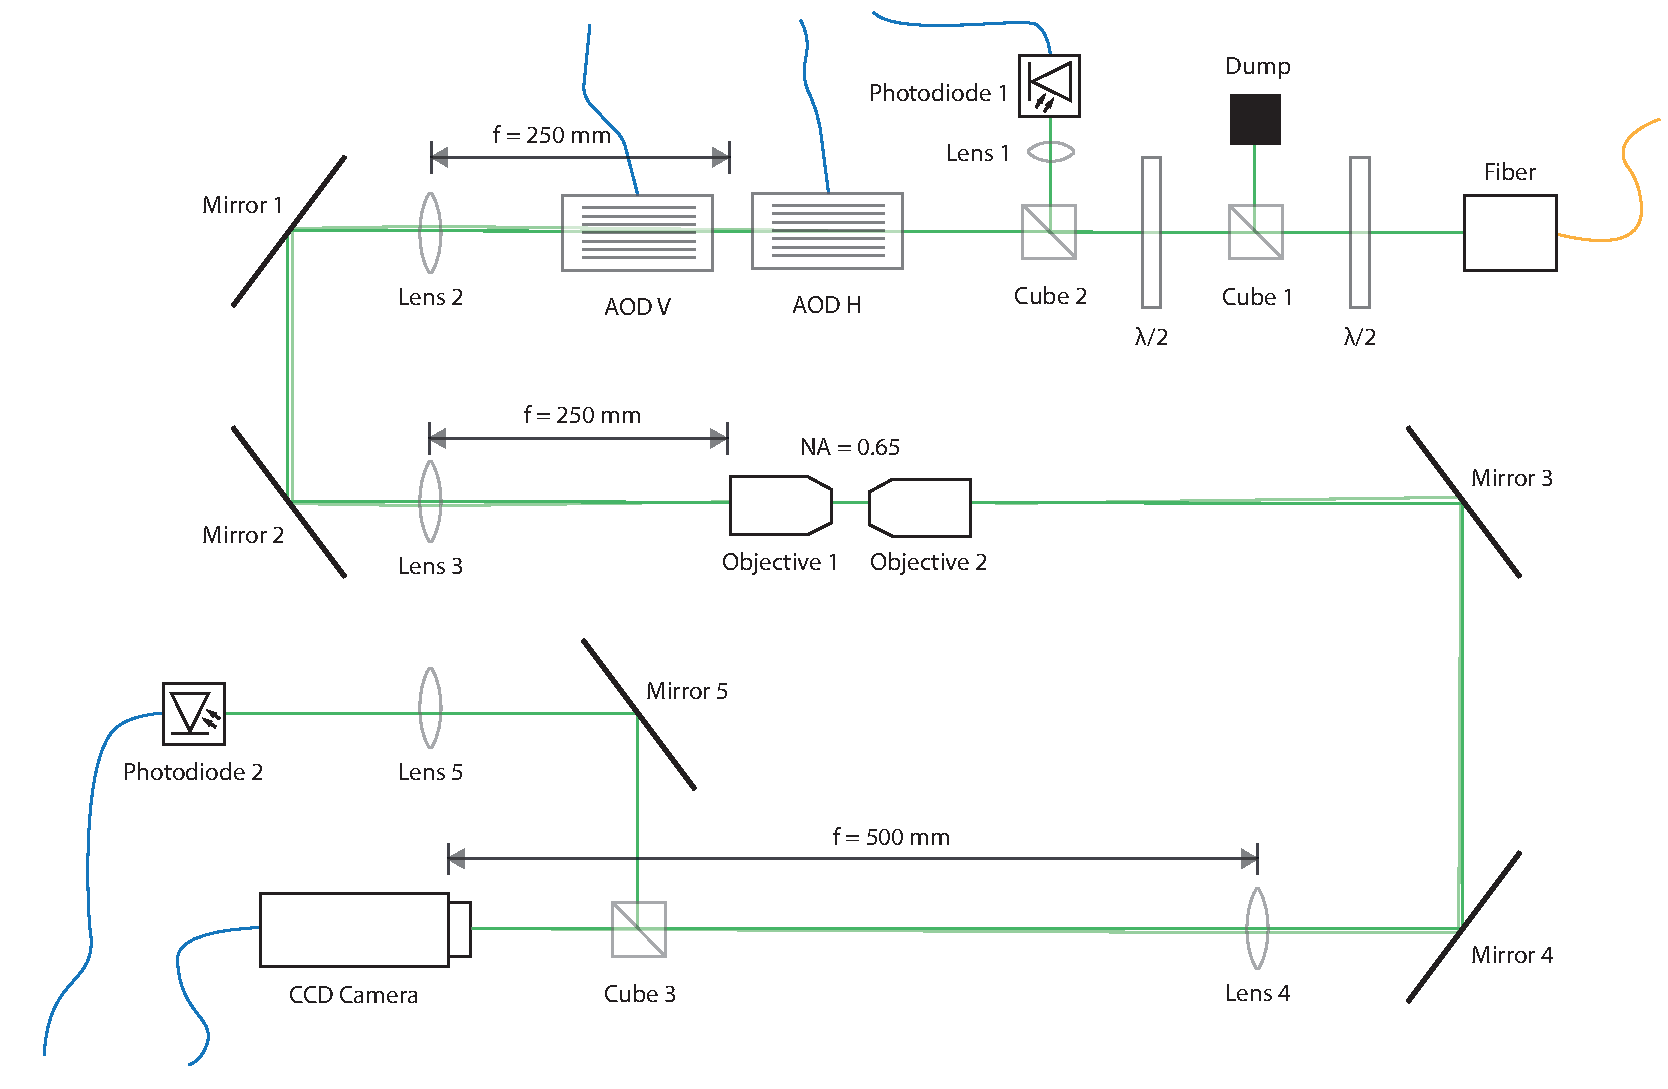
\includegraphics[width=\textwidth]{\figuredir{setup/beam-deflection.pdf}}
  \caption{Optical configuration of the beam deflection section.
  }\label{fig:setup_beam_deflection}
\end{figure}
For horizontal and vertical beam deflection two \gls{aod}s are used. A $1:1$
telescope comprised of two Lens 2 and Lens 3 projects the beam on a pair of
objectives. The purpose of the objective is to focus the laser later on to the
atom plane. Consecutively the laser is reflected by Mirror 3 and Mirror 4 to
the part intended for detection. Lens Lens 4 acts as a camera lens and
projects the beam to infinite focus on to the \gls{ccd} camera sensor. Cube 3
forks a portion of the beam away from the \gls{ccd} camera on to Mirror 5 that
guides the beam towards Lens 5 in order to focus the beam onto Photodiode 2.

\section{Electronics}

Beforehand we described the optical setups used. Now we want to emphasize
on the electronics how they are integrated into the optical setup.

\subsection{Signal source}

\subsection{Signal amplifier}

We use three signal amplifiers with respective input from the signal sources
to have an output power of about $P=\SI{2}{\watt}$ required by the \gls{aod}s
and \gls{aom} for ideal operation. The used amplifiers offer a second input
for external amplitude modulation. In case of the \gls{aom} we connect this
input to the intensity controller.

\subsection{Intensity controller}

The intensity controller is connected to Photodiode 1 in
\Cref{fig:setup_beam_deflection} that converts the laser power to a voltage
signal which we supply to the controller. Given the input signal we can
configure the controller for a reference input voltage. The controller will
then compare the input voltage with set reference voltage and output an error
signal that is proportional to the deviation of the input from the reference
voltage. The inverted error signal is feed to the signal amplifier connected
with the \gls{aom}.

\subsection{Trigger source}

To syncronize the signal sources, the \gls{ccd} camera and the oscilloscope
it was necessary to design a global trigger source that outputs a rising edge
signal to multiple devices and exposes a network programable interface.
The schematics and board layout can be found in the
\Cref{app:electronics:trigger_hub}.
